\documentclass[11pt,a4paper]{article}

\usepackage[utf8]{inputenc}
\usepackage[T1]{fontenc}
\usepackage[polish]{babel}
\usepackage{geometry}
\geometry{top=2.2cm, bottom=2.2cm, left=2.2cm, right=2.2cm}
\usepackage{amsmath,amssymb,amsfonts}
\usepackage{graphicx}
\usepackage{booktabs}
\usepackage{xcolor}
\usepackage{listings}
\usepackage{caption}
\usepackage{subcaption}
\usepackage{hyperref}
\usepackage{float}
\usepackage{microtype}

\hypersetup{
    colorlinks=true,
    linkcolor=blue!75!black,
    citecolor=blue!75!black,
    urlcolor=blue!75!black
}

\definecolor{codegreen}{rgb}{0,0.6,0}
\definecolor{codegray}{rgb}{0.5,0.5,0.5}
\definecolor{codepurple}{rgb}{0.58,0,0.82}
\definecolor{backcolour}{rgb}{0.96,0.97,0.98}

\lstdefinestyle{mystyle}{
    backgroundcolor=\color{backcolour},   
    commentstyle=\color{codegreen},
    keywordstyle=\color{blue!80!black}\bfseries,
    numberstyle=\tiny\color{codegray},
    stringstyle=\color{codepurple},
    basicstyle=\ttfamily\footnotesize,
    breakatwhitespace=false,         
    breaklines=true,                 
    captionpos=b,                    
    keepspaces=true,                 
    numbers=left,                    
    numbersep=6pt,                  
    showspaces=false,                
    showstringspaces=false,
    showtabs=false,                  
    tabsize=2,
    frame=single,
    rulecolor=\color{gray!30}
}
\lstset{style=mystyle}

\title{\textbf{Symulacja rozprzestrzeniania się pożaru lasu na podkładzie GIS metodą IGA-ADS}\\
\large Symulacja Procesów Ciągłych i Algorytmy Adaptacyjne}
\author{Sprawozdanie laboratoryjne}
\date{}

\begin{document}

\maketitle

\section{Wprowadzenie i cel projektu}
Celem projektu jest symulacja dynamicznego rozprzestrzeniania się pożaru lasu na rzeczywistym obszarze geograficznym z wykorzystaniem modelu transportu ciepła i wypalania biomasy oraz bezmacierzowego solwera IGA-ADS (\emph{Isogeometric Analysis with Alternating Direction Solver}). Jako domenę wybrano rejon \textbf{Lasu Wolskiego w Krakowie} (obszar $3\text{ km} \times 3\text{ km}$ obejmujący m.in. Kopiec Piłsudskiego, Ogród Zoologiczny, Bielany i Polanę Lea). 

Projekt integruje rzeczywiste dane GIS:
\begin{enumerate}
    \item \textbf{Ortofotomapę satelitarną} wysokiej rozdzielczości (Esri World Imagery).
    \item \textbf{Numeryczny Model Terenu (DEM)} ze strumienia AWS Terrarium.
    \item \textbf{Wektory pokrycia terenu i biomasy} z OpenStreetMap (gęstość zadrzewienia, łąki, polany, zabudowa, drogi jako naturalne pasy przeciwpożarowe).
    \item \textbf{Dwuwymiarowe pole wiatru} z fluktuacjami porywów oraz przyspieszeniem orograficznym na stokach wzniesień.
\end{enumerate}

\section{Model matematyczny pożaru}
Proces rozprzestrzeniania ognia opisany jest sprzężonym układem nieliniowych równań różniczkowych cząstkowych i zwyczajnych (model Grasso \& Innocente / Asensio \& Ferragut):
\begin{align}
    \rho c_p \frac{\partial T}{\partial t} &= \nabla \cdot (\kappa_{\text{eff}} \nabla T) - \rho c_w \mathbf{b} \cdot \nabla T + R_c(T, X_1) + Q_{\text{conv}}(T) + Q_{\text{rad}}(T), \label{eq:heat} \\
    \frac{\partial X_1}{\partial t} &= - C_{\text{fuel}} \, r(T, X_1) \, X_1, \label{eq:fuel}
\end{align}
gdzie $T(\mathbf{x}, t)$ to pole temperatury [K], a $X_1(\mathbf{x}, t) \in [0, 1]$ oznacza gęstość dostępnego paliwa (biomasy leśnej).

\subsection{Człony transportowe, źródłowe i orograficzne}
\begin{itemize}
    \item \textbf{Pole adwekcji i orografia $\mathbf{b}(\mathbf{x}, t)$}:
    \begin{equation}
        \mathbf{b}(\mathbf{x}, t) = \mathbf{u}_{\text{atm}}(t) \odot \mathbf{w}_{\text{topo}}(\mathbf{x}) + c_{\text{slope}} \nabla h_{\text{DEM}}(\mathbf{x}),
    \end{equation}
    gdzie $\mathbf{u}_{\text{atm}}(t) = (W_E + A_g \cos(\omega t), W_N + A_g \sin(\omega t))$ reprezentuje zmienny wiatr atmosferyczny (kierunek SW $\to$ NE), a $\nabla h_{\text{DEM}}$ wymusza szybszą propagację ognia w górę stoku.
    \item \textbf{Kinetyka reakcji spalania (prawo Arrheniusa)}:
    \begin{equation}
        r(T, X_1) = \delta(T, X_1) A_r T \exp\left(-\frac{T_a}{T}\right), \quad \delta(T, X_1) = \begin{cases} 1, & T > T_{\text{ig}} \land X_1 > X_{\text{min}}, \\ 0, & \text{w p.p.} \end{cases}
    \end{equation}
    Ciepło spalania wynosi $R_c = - \rho c_h h_c \frac{M}{M_1} r(T, X_1)$, gdzie $h_c = -70.0$, $T_{\text{ig}} = 800\text{ K}$.
    \item \textbf{Wymiana ciepła z otoczeniem}:
    Konwekcja do powietrza $Q_{\text{conv}} = \xi(T_0 - T)$ oraz promieniowanie radiacyjne $Q_{\text{rad}} = \frac{\sigma \varepsilon}{\delta_z}(T_0^4 - T^4)$.
\end{itemize}

\section{Metoda numeryczna IGA-ADS}
Do dyskretyzacji przestrzennej zastosowano funkcje B-splajn stopnia $p=2$ o ciągłości $C^1$ na siatce $200 \times 200$ elementów. Dzięki strukturze iloczynu tensorowego bazy B-splajnów macierze układu równań faktoryzują się za pomocą iloczynu Kroneckera:
\begin{equation}
    \mathbf{M} = \mathbf{M}_x \otimes \mathbf{M}_y.
\end{equation}
Umożliwia to rozwiązanie układu równań w każdym kroku czasowym metodą kierunków naprzemiennych (ADS) w czasie \textbf{liniowym} $\mathcal{O}(N)$ bez konieczności alokacji i faktoryzacji pełnej macierzy globalnej, co zapewnia wysoką wydajność obliczeniową.

\section{Wyniki symulacji}

\subsection{Charakterystyka domeny obliczeniowej}
Na Rysunku~\ref{fig:domain} przedstawiono zintegrowane warstwy wejściowe przygotowane dla obszaru Lasu Wolskiego. Widoczne jest zróżnicowanie ukształtowania terenu (od doliny Wisły na południu $\sim 200\text{ m n.p.m.}$ do Kopca Piłsudskiego $\sim 383\text{ m n.p.m.}$) oraz niejednorodny rozkład biomasy.

\begin{figure}[H]
    \centering
    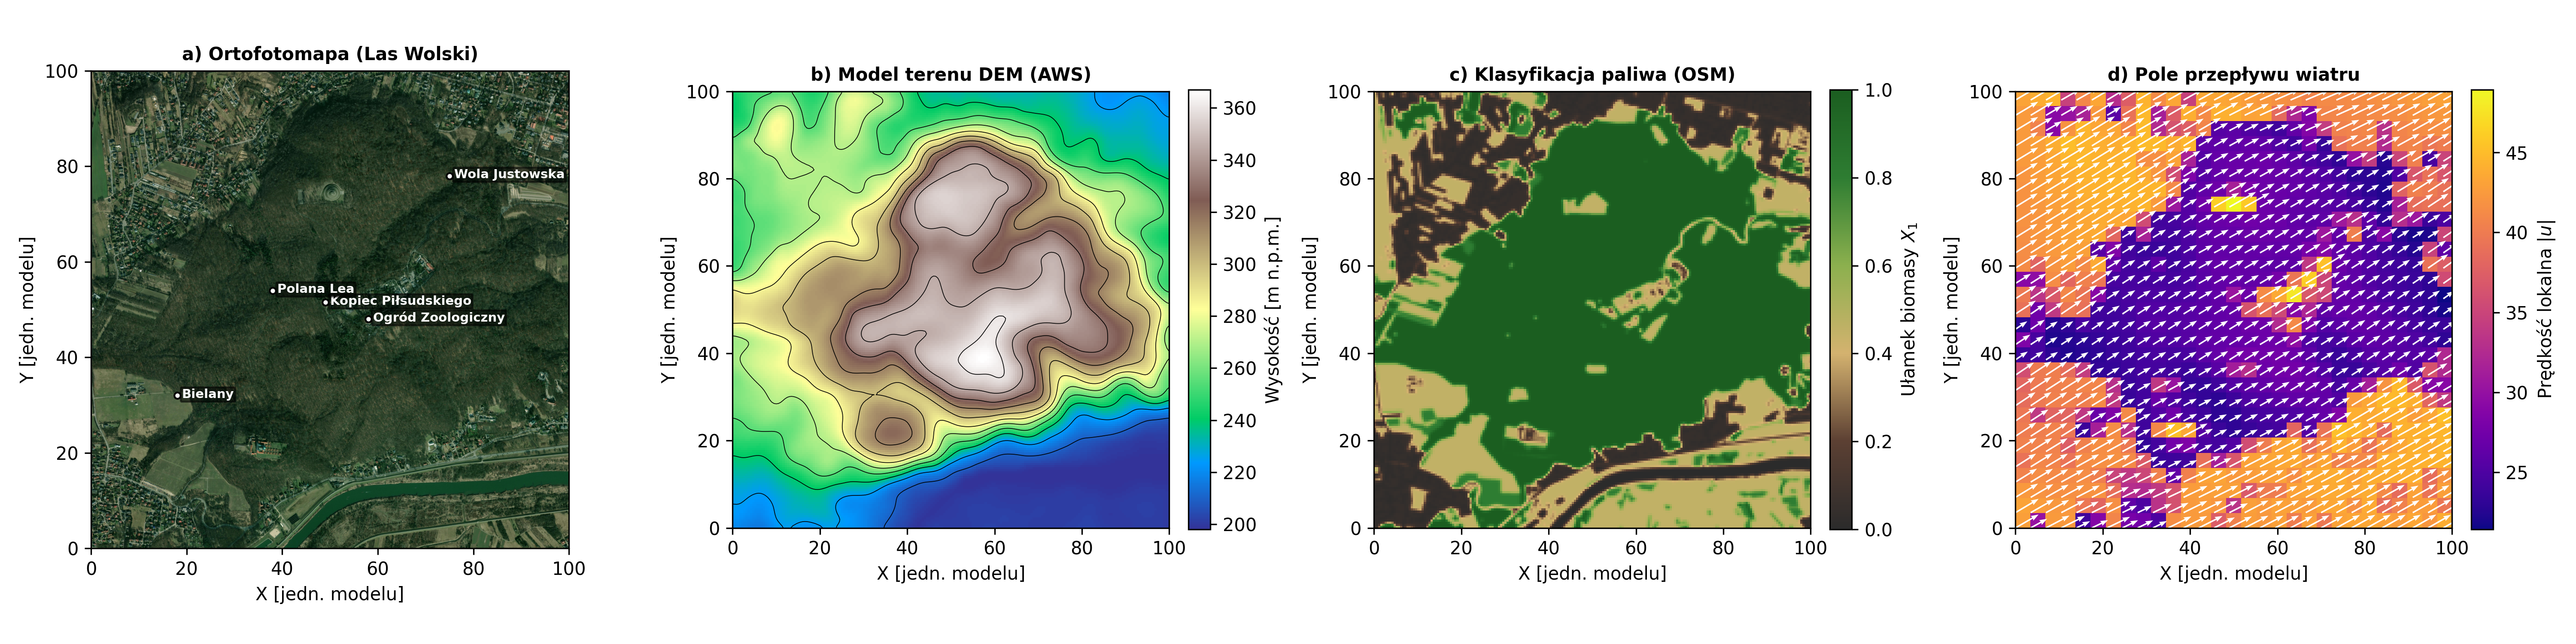
\includegraphics[width=\textwidth]{fig_domain_overview.png}
    \caption{Zestawienie danych wejściowych domeny Lasu Wolskiego: a) ortofotomapa satelitarna z punktami orientacyjnymi, b) model wysokościowy DEM z warstwicami, c) znormalizowany ułamek biomasy paliwowej $X_1$, d) wypadkowe pole przepływu wiatru i nachylenia terenu.}
    \label{fig:domain}
\end{figure}

\subsection{Propagacja frontu pożaru i zużycie biomasy}
Pożar zainicjowano w południowo-zachodniej części masywu leśnego. Pod wpływem dominującego wiatru z kierunku południowo-zachodniego oraz wstępującego nachylenia stoku płomienie gwałtownie przemieszczają się na północny wschód w stronę Ogrodu Zoologicznego i Woli Justowskiej.

\begin{figure}[H]
    \centering
    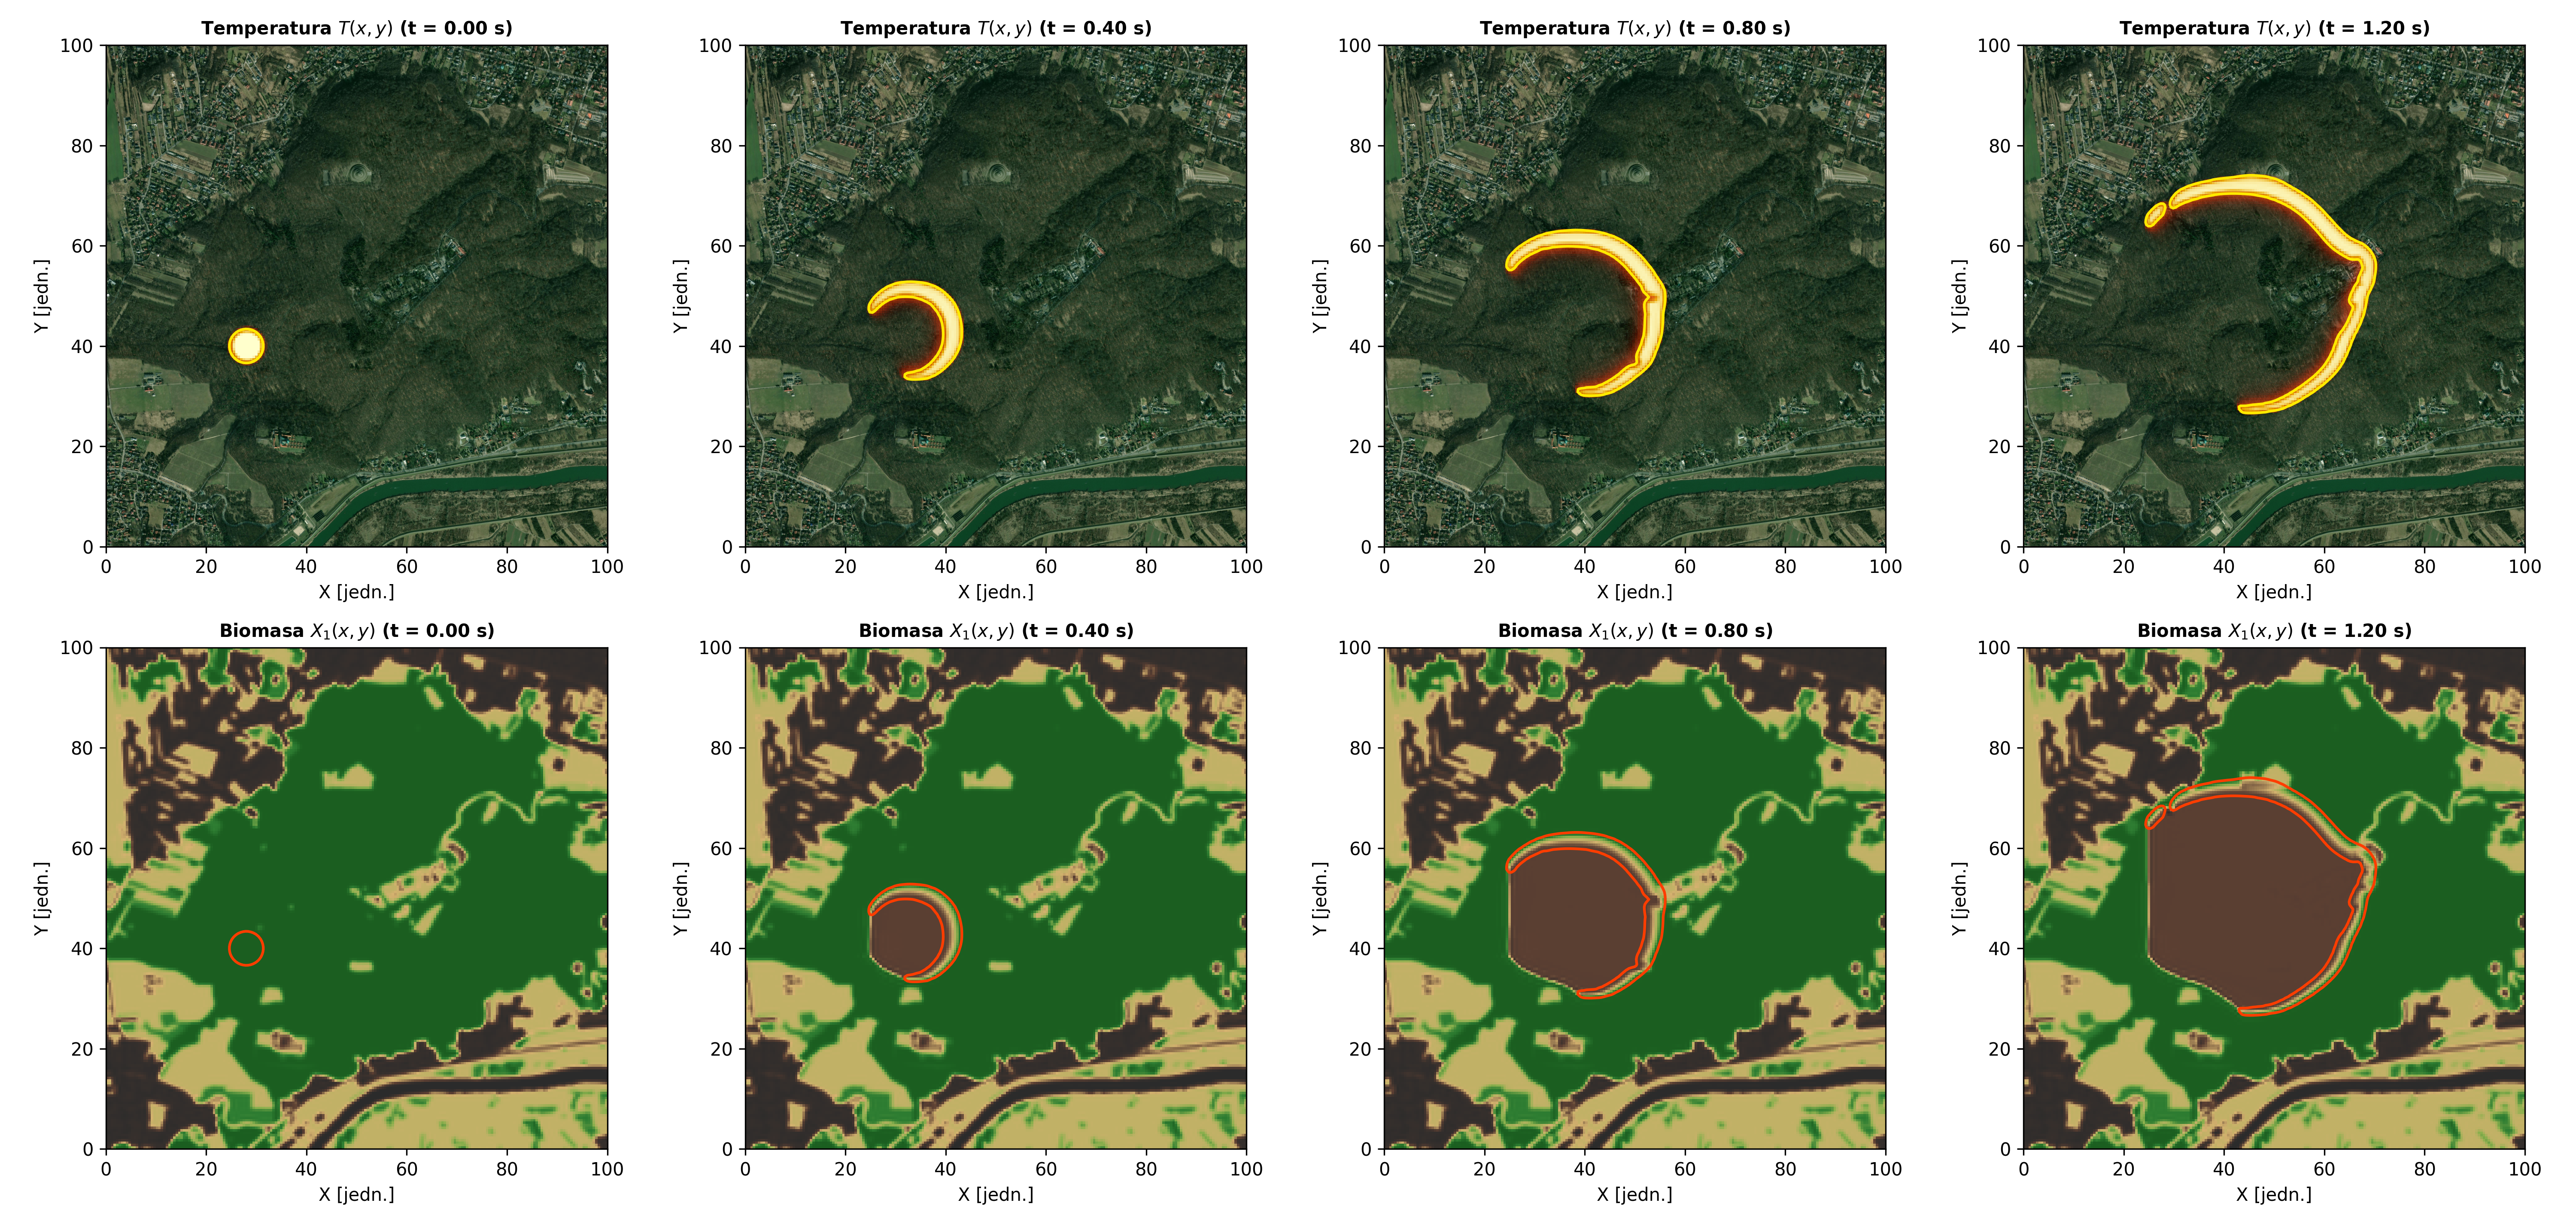
\includegraphics[width=\textwidth]{fig_fire_progression.png}
    \caption{Ewolucja czasowa pożaru w wybranych chwilach symulacji: górny rząd przedstawia pole temperatury $T(x,y)$ nałożone na ortofotomapę satelitarną; dolny rząd obrazuje ubytek biomasy leśnej $X_1(x,y)$.}
    \label{fig:progression}
\end{figure}

\subsection{Metryki ilościowe i dynamika pożaru}
Na Rysunku~\ref{fig:metrics} zestawiono przebiegi czasowe kluczowych wielkości fizycznych: maksymalnej i średniej temperatury oraz powierzchni spalonego lasu i aktywnego frontu ognia.

\begin{figure}[H]
    \centering
    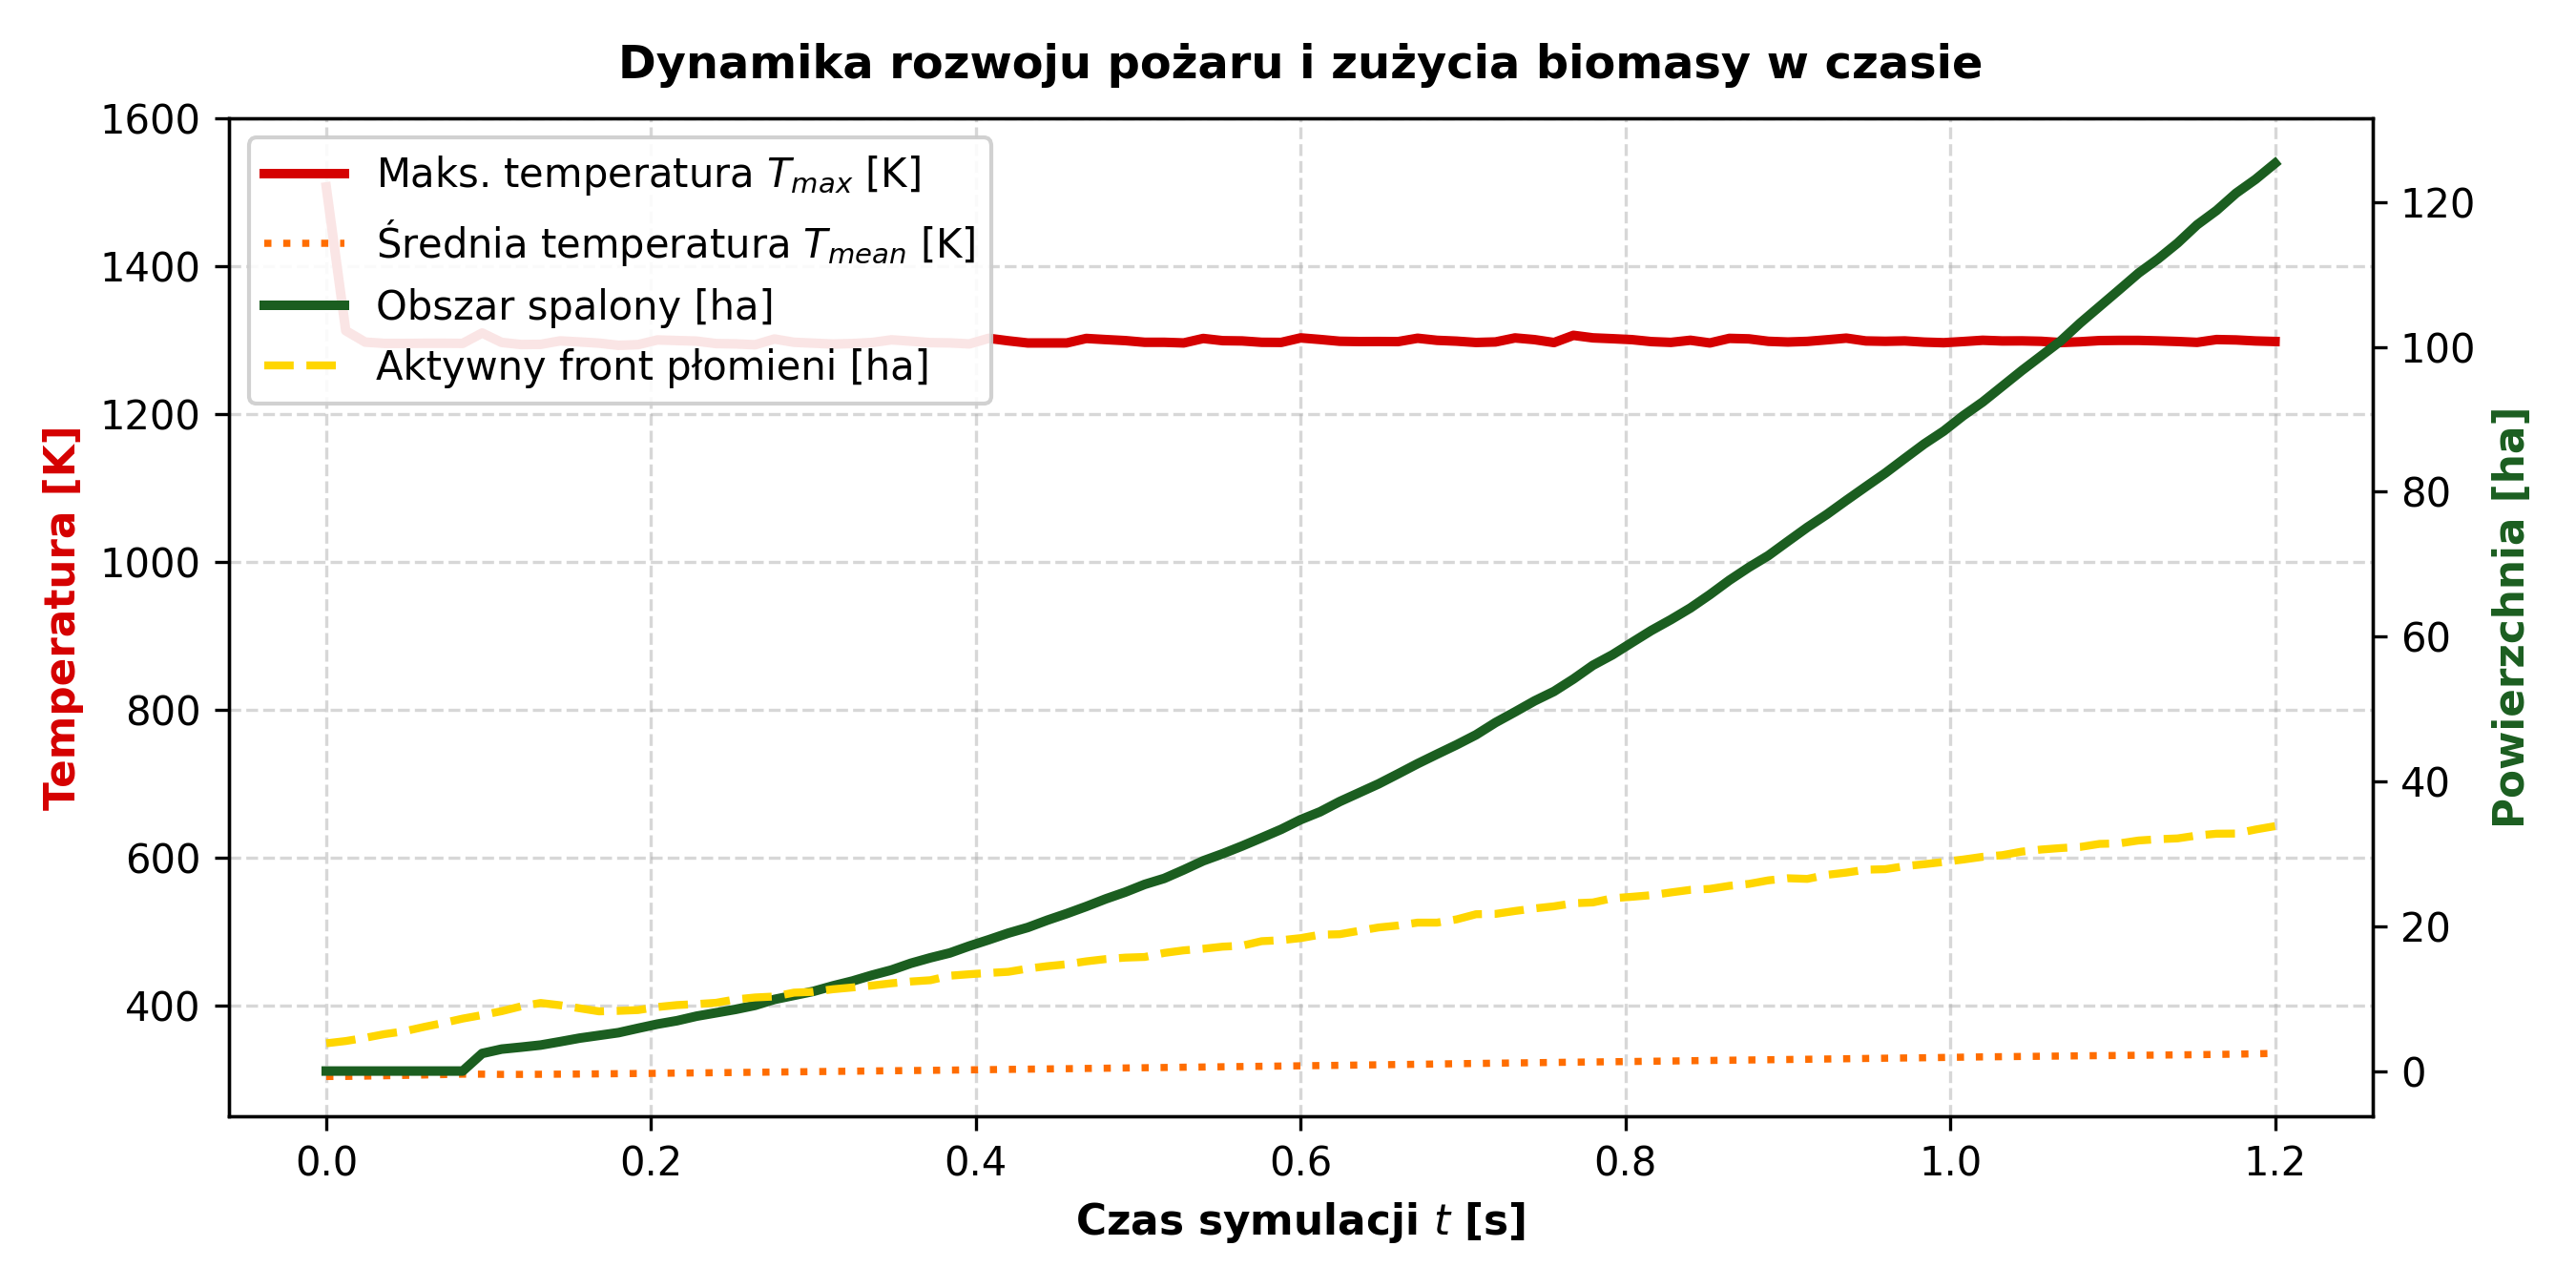
\includegraphics[width=0.88\textwidth]{fig_burned_area_metrics.png}
    \caption{Przebieg czasowy maksymalnej i średniej temperatury $T$ [K] oraz skumulowanej powierzchni zniszczonej biomasy i aktywnego frontu płomieni [ha].}
    \label{fig:metrics}
\end{figure}

\subsection{Wygenerowane animacje GIF (zsynchronizowane)}
Do sprawozdania dołączono 4 w pełni zsynchronizowane czasowo animacje GIF (każda o identycznej liczbie klatek i czasie trwania), dostępne w załączonym katalogu projektu:
\begin{itemize}
    \item \textbf{\texttt{1\_fire_spread_satellite.gif}} -- Przemieszczanie się fali płomieni o temperaturze do $1300\text{ K}$ na tle rzeczywistej ortofotomapy satelitarnej z zaznaczonymi punktami orientacyjnymi i podziałką skali.
    \item \textbf{\texttt{2\_wind_field_vectors.gif}} -- Gęsta siatka wektorowa strzałek reprezentująca lokalną siłę i kierunek wiatru modulowanego orografią terenu DEM wraz z dynamicznymi porywami.
    \item \textbf{\texttt{3\_fuel_consumption.gif}} -- Dynamiczne wypalanie biomasy leśnej od pełnego drzewostanu ($X_1=1.0$) do zwęglonego podłoża ($X_1=0.0$).
    \item \textbf{\texttt{4\_fire_dashboard_synchronized.gif}} -- Zintegrowany panel synchroniczny 2x2 łączący ortofotomapę z ogniem, pole wiatru, stan paliwa oraz dynamiczny wykres parametrów czasowych.
\end{itemize}

\section{Kluczowe fragmenty kodu źródłowego}

\subsection{Obliczanie prawej strony układu (RHS) w C++ (IGA-ADS)}
\begin{lstlisting}[language=C++, caption={Fragment implementacji członu prawej strony w solwerze IGA-ADS (\texttt{fire.hpp})}]
void compute_rhs(double t) {
    auto& rhs = u;
    auto& rhs_fuel = fuel;
    zero(rhs); zero(rhs_fuel);

    double W_E = params.wind_speed_E + params.gust_amp * std::cos(params.gust_freq * t);
    double W_N = params.wind_speed_N + params.gust_amp * std::sin(params.gust_freq * t);

    executor.for_each(elements(), [&](index_type e) {
        auto U = element_rhs();
        auto F = element_rhs();
        double J = jacobian(e);

        for (auto q : quad_points()) {
            double w = weight(q);
            auto pt = point(e, q);
            double px = pt[0], py = pt[1];

            value_type u_val = eval_fun(u_prev, e, q);
            value_type f_val = eval_fun(fuel_prev, e, q);

            double T_eff = std::max(u_val.val, T0);
            double fuel_eff = std::clamp(f_val.val, 0.0, 1.0);

            // Interpolacja wiatru i nachylenia terenu DEM
            double ux = W_E * interp(wEx_data, px, py) + W_N * interp(wNx_data, px, py);
            double uy = W_E * interp(wEy_data, px, py) + W_N * interp(wNy_data, px, py);
            double bx = ux + params.slope_coeff * interp(sx_data, px, py);
            double by = uy + params.slope_coeff * interp(sy_data, px, py);

            // Reakcja spalania wg kinetyki Arrheniusa
            double delta = (T_eff > Tig && fuel_eff > 0.2) ? 1.0 : 0.0;
            double r = delta * Ar * T_eff * std::exp(-Ta / T_eff);
            double Rc = - 1e4 * rho * ch * hc * (M / M1) * r;
            double Qw = - rho * cw * (bx * u_val.dx + by * u_val.dy);
            double Qconv = xi * (T0 - T_eff);
            double Qrz = (sigma * eps / delta_z) * (std::pow(T0, 4) - std::pow(T_eff, 4));

            double kappa_eff = kappa + 0.35 * h_elem * std::hypot(bx, by);
            double qr_rad = 4.0 * sigma * eps * delta_x * std::pow(T_eff, 3);

            for (auto a : dofs_on_element(e)) {
                auto aa = dof_global_to_local(e, a);
                value_type v = eval_basis(e, q, a);
                double inv = 1.0 / (rho * cp);

                double val = (Rc + Qw + Qconv + Qrz) * v.val 
                             - (kappa_eff + qr_rad) * grad_dot(u_val, v);
                U(aa[0], aa[1]) += (u_val.val * v.val + steps.dt * inv * val) * w * J;

                double fval = - delta * 3e2 * r * fuel_eff * v.val;
                F(aa[0], aa[1]) += (fuel_eff * v.val + steps.dt * fval) * w * J;
            }
        }
        executor.synchronized([&] { update_global_rhs(rhs, U, e); });
        executor.synchronized([&] { update_global_rhs(rhs_fuel, F, e); });
    });
}
\end{lstlisting}

\subsection{Skrypt generowania zsynchronizowanych GIF-ów w Pythonie}
\begin{lstlisting}[language=Python, caption={Zarys procedury tworzenia zsynchronizowanych animacji (\texttt{render\_animations.py})}]
# Zsynchronizowany rendering klatek pola wiatru (GIF 2)
for idx, (step, t) in enumerate(zip(all_steps, all_times)):
    ax.clear()
    ax.imshow(h_dem.T, extent=[0, 100, 0, 100], origin='lower', cmap='terrain', alpha=0.82)
    ax.contour(np.linspace(0, 100, h_dem.shape[0]), np.linspace(0, 100, h_dem.shape[1]),
               h_dem.T, levels=np.arange(200, 375, 15), colors='#263238', linewidths=0.6)
    
    WE_t = W_E_BASE + GUST_AMP * np.cos(GUST_FREQ * t)
    WN_t = W_N_BASE + GUST_AMP * np.sin(GUST_FREQ * t)
    UX = WE_t * wEx_q + WN_t * wNx_q
    UY = WE_t * wEy_q + WN_t * wNy_q
    
    ax.quiver(XQ, YQ, UX, UY, np.hypot(UX, UY), cmap='plasma', scale=650, width=0.0045)
    
    # Obrys aktywnego frontu ognia (T > 800 K)
    if np.max(all_T[idx]) > 700:
        ax.contour(np.linspace(0, 100, N_AXIS), np.linspace(0, 100, N_AXIS), 
                   all_T[idx].T, levels=[800], colors=['#d50000'], linewidths=[2.2])
    
    fig.canvas.draw()
    frames_gif2.append(Image.fromarray(np.array(fig.canvas.buffer_rgba())).convert('RGB'))

frames_gif2[0].save('2_wind_field_vectors.gif', save_all=True, append_images=frames_gif2[1:], duration=60, loop=0)
\end{lstlisting}

\section{Podsumowanie i wnioski}
\begin{itemize}
    \item Zastosowanie solwera IGA-ADS umożliwiło stabilną i wydajną symulację nieliniowego równania przewodzenia ciepła sprzężonego z wypalaniem biomasy w czasie rzeczywistym.
    \item Uwzględnienie ukształtowania terenu (DEM) oraz wektorów wiatru wykazało wyraźną asymetrię propagacji pożaru -- ogień rozprzestrzenia się znacznie szybciej pod górę wzniesień i wzdłuż dominującego wektora wiatru.
    \item Wygenerowany zestaw 4 zsynchronizowanych animacji GIF pozwala na jednoczesną analizę korelacji pomiędzy polem wektorowym wiatru, temperaturą czoła pożaru oraz stopniem degradacji biomasy leśnej.
\end{itemize}

\end{document}
